% file: 3-7-sssp/bellman-ford-negative-cycle.tex

\documentclass[tikz]{standalone}
\usetikzlibrary{shapes, positioning}

\begin{document}
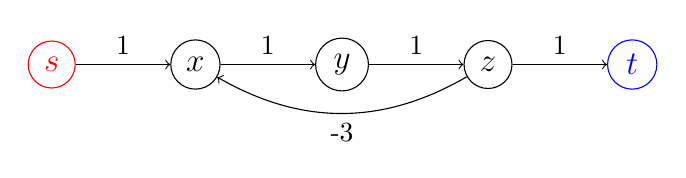
\begin{tikzpicture}[v/.style = {draw, circle, minimum size = 8pt, font = \large},
    node distance = 1.2cm,
    every edge/.style = {draw, ->},
    w/.style = {above}]
  \node (s) [v, red] {$s$};

  \node (x) [v, right = of s] {$x$};
  \node (y) [v, right = of x] {$y$};
  \node (z) [v, right = of y] {$z$};
  \node (t) [v, right = of z, blue] {$t$};

  \path (s) edge node[w] {1} (x)
	(x) edge node[w] {1} (y)
	(y) edge node[w] {1} (z)
	(z) edge node[w] {1} (t)
	    edge[bend left] node[below] {-3} (x);
\end{tikzpicture}
\end{document}
